%HW07.tex
%
% Seventh Homework for Graduate Algebra
% Frank Sottile
%%%%%%%%%%%%%%%%%%%%%%%%%%%%%%%%%%%%%%%%%%%%%%%%%%%%%%%%%%%%%%%%%%%%%%%
\documentclass[12pt]{article}
\usepackage{multicol,amsfonts, amssymb,  mathtools,amsmath}
\usepackage{colordvi,graphicx}
\headheight=8pt
%
\topmargin=-95pt
\textheight=740pt   \textwidth=570pt
\oddsidemargin=-65pt \evensidemargin=-65pt

\pagestyle{empty}

%%%%%%%%%%%%%%%%%%%%%%%%%%%%%%%%%%%%%%%%%%%%
\newcommand{\CC}{{\mathbb C}}
\newcommand{\KK}{{\mathbb K}}
\newcommand{\NN}{{\mathbb N}}
\newcommand{\QQ}{{\mathbb Q}}
\newcommand{\RR}{{\mathbb R}}
\newcommand{\TT}{{\mathbb T}}
\newcommand{\ZZ}{{\mathbb Z}}

\newcommand{\calA}{{\mathcal A}}
\newcommand{\be}{{\bf e}}
\newcommand{\bfi}{{\bf i}}
\newcommand{\bfj}{{\bf j}}

\newcommand{\Hom}{\mbox{Hom}}
\newcommand{\Aut}{\mbox{Aut}}
\newcommand{\spec}{\mbox{spec}}
\newcommand{\cone}{\mbox{cone}}

\newcommand{\vect}[2]{(\begin{smallmatrix}#1\\#2\end{smallmatrix})}
\newcommand{\msp}{\hspace{8pt}}
%\newcommand{\Square}{\raisebox{-2pt}{\includegraphics{images/Square.eps}}}
\newcommand{\Square}{\raisebox{-2pt}{\Large$\square$}}

\def\Color#1#2{\special{color push cmyk #1}#2\special{color pop}}
%\def\Indigo#1{\Color{.42 1. 0. .49}{#1}}
\def\Indigo#1{\Color{1. .95 .05 .4}{#1}}
\def\MyViolet#1{\Color{.6 1. 0. .15}{#1}}
\def\TAMU#1{\Color{.15 1. .39 .69}{#1}}

\newcommand{\barsl}{\noindent\begin{minipage}[t]{590pt}
\Indigo{\rule{590pt}{1.2pt}}\vspace{-5.7mm}\\
\MyViolet{\rule{590pt}{1.2pt}}\vspace{-5.7mm}\\
\Blue{\rule{590pt}{1.2pt}}\vspace{-5.7mm}\\
\Green{\rule{590pt}{1.2pt}}\vspace{-5.7mm}\\
\Yellow{\rule{590pt}{1.2pt}}\vspace{-5.7mm}\\
\Orange{\rule{590pt}{1.2pt}}\vspace{-5.7mm}\\
\Red{\rule{590pt}{1.2pt}}\bigskip
\end{minipage}}


\newcommand{\barsn}{\noindent\begin{minipage}[t]{590pt}
\Indigo{\rule{590pt}{1.1pt}}\vspace{-4.5mm}\\
\MyViolet{\rule{590pt}{1.1pt}}\vspace{-4.5mm}\\
\Blue{\rule{590pt}{1.1pt}}\vspace{-4.5mm}\\
\Green{\rule{590pt}{1.1pt}}\vspace{-4.5mm}\\
\Yellow{\rule{590pt}{1.1pt}}\vspace{-4.5mm}\\
\Orange{\rule{590pt}{1.1pt}}\vspace{-4.5mm}\\
\Red{\rule{590pt}{1.1pt}}\bigskip
\end{minipage}}

\def\demph#1{\TAMU{{\sl #1}}}
\def\defcolor#1{\TAMU{#1}}

\begin{document}
\LARGE 
\noindent
Algebra \ \ Autumn 2025\vspace{1pt}\\
Frank Sottile\vspace{2pt}\\
\Large 9 October 2025 \hfill
\sf
 Seventh Homework\makebox[20pt][l]{\ }
\normalsize\vspace{10pt}

\noindent
Write your answers neatly, in complete sentences.  
I highly recommend recopying your work before handing it in.
Correct and crisp proofs are greatly appreciated; oftentimes your work can be shortened and made clearer.

\barsn

\noindent\Maroon{{\sf Hand in at the start of class, Thursday 16 October:}} 


\begin{enumerate}
\setcounter{enumi}{36}

%%%%%%%%%%%%%%%%%%%%%%%%%%%%%%%%%%%%%%%%%%%%%%%%%%%%%%%%%%%%%%%%%%%%%%%%%%%%%%%%%%%%%%%%%%%%%%%%%%%%
\item  Let $G$ be a group of order 3825.
  Prove that if $H$ is a normal sugroup of $G$ of order 17, then $H$ is a subgroup of the center of $G$.
%%%%%%%%%%%%%%%%%%%%%%%%%%%%%%%%%%%%%%%%%%%%%%%%%%%%%%%%%%%%%%%%%%%%%%%%%%%%%%%%%%%%%%%%%%%%%%%%%%%%

%%%%%%%%%%%%%%%%%%%%%%%%%%%%%%%%%%%%%%%%%%%%%%%%%%%%%%%%%%%%%%%%%%%%%%%%%%%%%%%%%%%%%%%%%%%%%%%%%%%%
\item  Which group of order 8 is $(S_2)^2\rtimes S_2$ ?  
%%%%%%%%%%%%%%%%%%%%%%%%%%%%%%%%%%%%%%%%%%%%%%%%%%%%%%%%%%%%%%%%%%%%%%%%%%%%%%%%%%%%%%%%%%%%%%%%%%%%

%%%%%%%%%%%%%%%%%%%%%%%%%%%%%%%%%%%%%%%%%%%%%%%%%%%%%%%%%%%%%%%%%%%%%%%%%%%%%%%%%%%%%%%%%%%%%%%%%%%%
\item   Let $N\vcentcolon= \ZZ_2\oplus\ZZ_2$.
  Determine $\Aut(N)$ and identify the group $N\rtimes \Aut(N)$.
%%%%%%%%%%%%%%%%%%%%%%%%%%%%%%%%%%%%%%%%%%%%%%%%%%%%%%%%%%%%%%%%%%%%%%%%%%%%%%%%%%%%%%%%%%%%%%%%%%%%


%%%%%%%%%%%%%%%%%%%%%%%%%%%%%%%%%%%%%%%%%%%%%%%%%%%%%%%%%%%%%%%%%%%%%%%%%%%%%%%%%%%%%%%%%%%%%%%%%%%%
\item  Universal constructions are uniquely isomorphic.
  \begin{enumerate}
    \item Let $S$ be a set and suppose that the abelian group $A$ is free on $S$.         
          If $A'$ is another abelian group that is free on $S$, show that there is a unique isomorphism 
          from $A$ to $A'$, as abelian groups that are free on $S$.

        \item Let $M$ be a commutative monoid with Grothendieck group $K(M)$ and suppose that $G$ is a group with a map
            $M\to G$ such that for any abelian group $B$, the pullback map
          \[
          \Hom_{\rm ab-gp}(G,B)\ \longrightarrow\ \Hom_{\rm monoid}(M,B)
          \]
          is a bijection.
          Show that there is a unique isomorphism $K(M)\to G$ that preserves this universal property. 
      
\end{enumerate}          
%%%%%%%%%%%%%%%%%%%%%%%%%%%%%%%%%%%%%%%%%%%%%%%%%%%%%%%%%%%%%%%%%%%%%%%%%%%%%%%%%%%%%%%%%%%%%%%%%%%%



%%%%%%%%%%%%%%%%%%%%%%%%%%%%%%%%%%%%%%%%%%%%%%%%%%%%%%%%%%%%%%%%%%%%%%%%%%%%%%%%%%%%%%%%%%%%%%%%%%%%
%  
\item \Maroon{{\large Groups of Order Twelve.}}
Recall: if $p\neq q$ prime numbers, all groups of order $p^2q$ have a normal Sylow subgroup.



\begin{enumerate}

\item Determine all groups of orders 3 and 4, along with their groups of automorphisms.

\item Let $G$ be a group of order twelve, and set $N_2$ and $N_3$ to be 2- and 3-Sylow subgroups.
  Show that $G=N_2 N_3$ and deduce that $G$ is a semi-direct product (in some order, $N_2\rtimes N_3$ or $N_3\rtimes N_2$)
  of its Sylow subgroups.

\item  Using the previous two questions, determine all possible groups of order twelve, up to isomorphism.
  That is, consider all possible semi-direct products and identify those which are isomnorphic

\item You have seen a few groups of order twelve, namely $\ZZ_{12}$, $\ZZ_4\oplus \ZZ_3$, $\ZZ_2\oplus \ZZ_6$,
  $D_{6}$, $\ZZ_2\times S_3$, and $A_4$.
  Identify these with groups you constructed as semi-direct products.
  Does one get all them?

      
\end{enumerate}
%%%%%%%%%%%%%%%%%%%%%%%%%%%%%%%%%%%%%%%%%%%%%%%%%%%%%%%%%%%%%%%%%%%%%%%%%%%%%%%%%%%%%%%%%%%%%%%%%%%%


%%%%%%%%%%%%%%%%%%%%%%%%%%%%%%%%%%%%%%%%%%%%%%%%%%%%%%%%%%%%%%%%%%%%%%%%%%%%%%%%%%%%%%%%%%%%%%%%%%%%
%
\item    A subset $X$ of an abelian group $F$ is \demph{linearly independent} if
  $n_1x_1+n_2x_2+\dotsb+n_kx_k=0$ implies that $n_i=0$ for all $i$, where
 $n_i\in\ZZ$ and $x_1,\dotsc,x_k$ are distinct elements of $X$.
 %%%%%%%%%%%%%%%%%%%%%%%%%%%%%%%%%%%%%%%%%%%%%%%%%%%%%%%%%%%%%%%%%%%%%%%%%%%%%%%%%%%%%%%%%%%%%%%%%%%
 \begin{enumerate}
  \item Show that $X$ is linearly independent if and only if every nonzero element of the
    subgroup $\langle X\rangle$ it generates may be written uniquely in the form
    $n_1x_1+\dotsb+n_kx_k$, where $n_i\in\ZZ$ and $x_1,\dotsc,x_k$ are distinct elements of
    $X$. 
  \item 
    Prove or give a counter example to the following statement:

    If  $F$ is free abelian of finite rank $n$, then  every
    linearly independent subset of $n$ elements is a basis.
    
  \item 
    Prove or give a counter example to the following statement:

     If $F$ is free abelian, then  every
     linearly independent subset of $F$ may be extended to a basis of $F$.
     
  \item 
    Prove or give a counter example to the following statement:

     If $F$ is free abelian, then every generating set
    of $F$ contains a basis of $F$.
 \vspace{-2pt}

 \end{enumerate}
%%%%%%%%%%%%%%%%%%%%%%%%%%%%%%%%%%%%%%%%%%%%%%%%%%%%%%%%%%%%%%%%%%%%%%%%%%%%%%%%%%%%%%%%%%%%%%%%%%%%  


 \end{enumerate}
%%%%%%%%%%%%%%%%%%%%%%%%%%%%%%%%%%%%%%%%%%%%%%%%%%%%%%%%%%%%%%%%%%%%%%%%%%%%%%%%%%%%%%%%%%%%%%%%%%%%  


\end{document}

%%%%%%%%%%%%%%%%%%%%%%%%%%%%%%%%%%%%%%%%%%%%%%%%%%%%%%%%%%%%%%%%%%%%%%%%%%%%%%%%%%%%%%%%%%%%%%%%%%%%
\item  
%%%%%%%%%%%%%%%%%%%%%%%%%%%%%%%%%%%%%%%%%%%%%%%%%%%%%%%%%%%%%%%%%%%%%%%%%%%%%%%%%%%%%%%%%%%%%%%%%%%%

